\chapter{Introduction}\label{ch:intro}

\section{Context}\label{sec:intro-context}

% historical context
As of 2022 humanity has developed tools for unprecedented growth in wealth and technology on a global scale \fakecite. In such times a great deal of consumerism and interconnection is present with people needing product produced faster and more consistently than ever \fakecite. 
As one would expect, this creates a high demand for manufacturers to reliably and consistently being able to provide products, while also remaining flexible, as the demand for different product change rapidly. 
% argue for why automation is better
% https://www.fishmancorp.com/robotics-manufacturing/
% https://www.universal-robots.com/blog/solving-complex-problems-with-innovative-concepts-and-robotic-solutions/
In order to provide great volumes of products, manual labor has is essential as assembly, transport and manipulation processes rely on these. Due to these types of manual labor being largely done by unskilled workers, automation alternatives are being adopted which provides benefits. 
% this is referred to as industry 4.0
% benefits for employer
These include for the employer: Avoid having to pay monthly salaries to unskilled labored individuals doing manual tasks, here the automation solution only requires electrical energy and potential supervision by a qualified individual. Potential risks are also involved when hiring humans as the workforce can be inconsistent due to human error\fakecite or left out due to illness etc. Considerations with regards workers rights such as working conditions and wage also needs not to be considered. These cause production limitations in the form of stand still hours, such as bathroom and lunch breaks along with after work hours and holidays. 
% benefits for the employee 
This replacement of manual labor also benefits the employee, as boring and physically wearing work is automated, enabling the employees to take on different and less wearing roles. While the issue of labor unemployment becomes apparent solutions which provide support to already hired workers have been developed, such as \gls{cobot}\fakecite. \medskip

% categories of problems in robotics for factories
When implementing automation of production lines using robotics, certain categories of problems are revealed. These include: Assembly, alteration and \gls{pnp}, the last being the one of interest in this project. 
\section{Problem Description}\label{sec:intro-problem-description}
% applications
Pick and place \gls{manipulator}s are used in a wide variety of different fields such as 
sorting of waste \cite*{robotic-pick-and-toss-facilitates-urban-waste-sorting}
handling of food \cite*{automation-of-mobile-pick-and-place-robotic-system-for-small-food-industry}\cite*{development-of-a-food-handling-soft-robot-hand-considering-a-high-speed-pick-and-place-task} and factory bin picking \cite*{real-time-industrial-bin-picking-with-a-hybrid-deep-learning-engineering-approach} \cite*{a-bin-picking-benchmark-for-systematic-evaluation-of-robotic-pick-and-place-systems} \cite{generic-development-of-bin-pick-and-place-system-based-on-robot-operating-system}. The solutions in these industries are examples of subcategories under the pick and place problem, namely sorting and bin picking. Since both of these are sub categories of the pick and place problem, they fundamentally follow the same sequential four phases from start to end. 
% All of these problems fundamentally contain the same structure as shared among all pick-and-place problems.
These steps being pre-grasping, grasping, transport, and placement \cite*{a-bin-picking-benchmark-for-systematic-evaluation-of-robotic-pick-and-place-systems} for traditional .
% pre-grasp
The pre-grasp phase involves localizing the object(s), potentially estimating their pose and executing the trajectory to move the end effectors grasp, collision free to said object(s). Here different potential grasp can be considered in order to determine the best pose for the end effector.
% grasping
In the grasping phase the end effector gasps the object in such a manner that the object's entire weight is supported by the \gls{ee}, and ends when the object no longer is in contact with the environment, which often is the container holding the object.
% transport
The transportation phase involves the motion of the manipulator to move from the pose achieved after the grasping phase, to a pose ready for placement of the object in the desired placing area or fixture. Here considerations may be needed with regards to how much force and torque the \gls{ee} can tolerate without losing the object.
% placement
Finally the goal of the placing phase is to place the object within the placing area or fixture in a desired end pose. Here the constraints on the end pose might differ significantly based on the application, as the pose of greens in a crate might need less precision than if the manipulator hands a bolt to the next robotics system in the pipeline. \medskip

While these phases make up a traditional \gls{pnp} systems, certain assumptions are made regarding the objects of interest in order for this pipeline to function. Specifically the localization and pose estimation of the pre-grasp phase are assumed possible due to \gls{cv} often being the sensory system for such tasks. Due to \gls{cv} techniques mimicking the human eye the field's maturity has generated a wide range solution proposals to these problems.


solutions to computer vision: classical,old fashion, deep learning based 

deep learning on transparent objects and reflective objects, shown less than ideal results

classical approaches% https://ieeexplore.ieee.org/abstract/document/7860048


vision has been used for many years \fakecite 


% traditional pipeline makes assumptions -> 

% ind end effector pose est
\section{Thesis Overview}\label{sec:intro-thesis-overview}































































% The developments in robotics as a field has over the past years provided automation solutions to execute repetitive manual tasks with high efficiency and reliability \fakecite. One of the most common tasks being pick and place tasks which involves picking un an object from one position and placing is in another. This is can be parted into the following subparts: Object localization, pose estimation, grasping and placing. In the solutions currently present for industrial use \gls{cv} is used for object localization and \gls{pe} due to the low cost of cameras and the fields maturity. However, while these solutions may be sufficient for certain tasks they fundamentally suffer from the weaknesses introduced by vision techniques. These include a great number of outliers caused by occlusions, reflecting, transparent or homogeneous surfaces, and repetitive structures when solving the \gls{corr-problem}. These problems as of the writing of this project have jet to be completely solved. Promising results have been found with the rise of \gls{dl} which in present time has proven its versatility and provides proof of concept solutions for narrow cases in pose estimation of transparent \cite{6dof-pose-estimation-of-transparent-object-from-a-single-rgb-d-image} and reflective \medskip

% \begin{minipage}{0.45\textwidth}
% 	objects \cite{6d-pose-estimation-of-objects:-recent-technologies-and-challenges}. This is relevant since industrial settings often contain transparent and especially reflecting objects as metallic parts tend to appear frequently and have high reflectances. To solve these problems this project aims to perform in-hand pose estimation through only the use of tactile sensors. Specifically this will be done on a Shadow Dexterous Hand \cite{shadow-dex-hand} with 20 \gls{dof}. Using tactile inputs rather than visual, eliminates the weaknesses mentioned above. A schematic showing the hand can be seen in \figref{fig:shadow-dex-hand-schematic}. Using this approach, the overall problem can be partitioned into 3 sub-problems labeled problem 1, 2 and 3. Problem 1 involves modeling the contact between the gripper's fingers and the object, also referred to as tactile perception. Problem 2 is to convert the collected data from problem 1 to meaningful surface data, treat these data as features and use them to estimate pose candidates. Finally problem 3 involves in-hand manipulation, such that further information is gained by probing the object. Here new desired surface points are found through intelligent probing such that strong surface features are found to better identify the object's correct pose. \medskip
% 	\end{minipage} 
% 	\hfill
% 	\begin{minipage}{0.45\textwidth}
% 	\begin{figure}[H]
% 		\begin{small}
% 			\begin{center}
% 				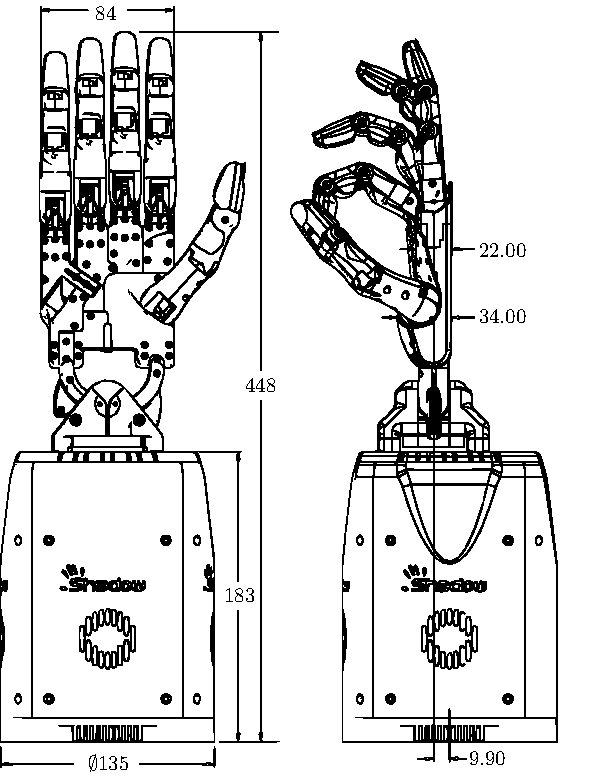
\includegraphics[width=0.95\textwidth]{chapters/introduction/fig/shadow-dex-hand-vector.pdf}
% 			\end{center}
% 			\caption{Schematic of Shadow Dexterous Hand from Shadow Robots, based on \cite{shadow-dex-hand-schematic}. The measurements are in \SI{}{\milli\metre}.}
% 			\label{fig:shadow-dex-hand-schematic}
% 		\end{small}
% 	\end{figure}
% \end{minipage}

% Thus the hypothesis of this projects $\text{H}_1$, will be testing if intelligent probing for strong features increases in-hand pose estimation performance, with the null hypothesis $\text{H}_0$ being that there is no statistical significant difference in the pose estimation performance of the system if the probing is done randomly or intelligently at a certainty level of \highlight{95\%}. Here pose estimation performance is quantified in terms of mean execution time for estimating the pose with an accuracy greater than \highlight{95\%}. \medskip

% The development of this project is done in the \gls{docker} provided by Shadow Robotics for simulation, control and development of the hand \cite{shadow-dex-github}. Here a hardware-simulation agnostic \gls{ros} \cite{ros} control \cite{ros-control} interface is found, which contains fundamental tools to interact with the robot hand. The dynamic simulation environment Gazebo \cite{gazebo} is likewise packaged as part of the \gls{docker} and is thus the one used for this project.
% To solve the problems presented, the \gls{ros} packages in \tabref{tab:software-package-table} will be applied, where \texttt{ros\_utils} and \texttt{in\_hand\_pose\_estimation} will be developed during this project.

% \begin{table}[h]
% 	\begin{small}
% 		\begin{center}
% 			\begin{tabular}[c]{ | l r | l | } \hline
% 				\cellcolor{tableheader} \textbf{Package}           & \cellcolor{tableheader} & \multicolumn{1}{l|}{\cellcolor{tableheader} \textbf{Description}} \\ \hline \hline
% 				\texttt{in\_hand\_pose\_estimation}                & \meta{meta} & \textbf{Project package of the in-hand pose estimation system} \\ \hline
% 				\hspace{0.3cm} \texttt{in\_hand\_pose\_estimation} &             & Integration of the full in-hand pose estimation pipeline  \\ \hline
% 				\hspace{0.3cm} \texttt{sr\_tactile\_image}         & \pkg{pkg}   & Extraction of tactile perception  \\ \hline
% 				\hspace{0.3cm} \texttt{sr\_pose\_estiamtion}       & \pkg{pkg}   & Estimate the pose of object based on tactile perception \\ \hline
% 				\hspace{0.3cm} \texttt{sr\_hand\_manipulation}     & \pkg{pkg}   & Manipulate object in hand to probe for strong features \\ \hline \hline
% 				\texttt{sr\_common}                                & \meta{meta} & \textbf{Shadow package for commonly used tools} \\ \hline
% 				\hspace{0.3cm} \texttt{sr\_common}                 &             & Implements commonly used tools such as messages \\ \hline
% 				\hspace{0.3cm} \texttt{sr\_robot\_msgs}            & \pkg{pkg}   & Messages used to communicate with the robot hand  \\ \hline 
% 				\hspace{0.3cm} \texttt{\dots}                      &             &  \\ \hline \hline
% 				\texttt{sr\_core}                                  & \meta{meta} & \textbf{Shadow package for core tools} \\ \hline
% 				\hspace{0.3cm} \texttt{sr\_core}                   &             & Implements core features of the hand such as hardware interfacing \\ \hline
% 				\hspace{0.3cm} \texttt{sr\_hand}                   & \pkg{pkg}   & Contains the hand commander for controlling the robot hand  \\ \hline
% 				\hspace{0.3cm} \texttt{\dots}                      &             &  \\ \hline \hline
% 				\texttt{ros\_utils}                                & \pkg{pkg}   & \textbf{Utilities for interfacing ROS/Gazebo/MoveIt/Eigen etc} \\ \hline
% 			\end{tabular}
% 		\end{center}
% 		\caption{Software packages used in the in-hand pose estimation system.}
% 		\label{tab:software-package-table}
% 	\end{small}
% \end{table}

% To present this work, the \gls{sota} solutions to each of the three problems described above will be presented in \chapref{ch:state-of-the-art}, where the best fitting methods for this use case will be chosen. In \chapref{ch:1-tactile-perception} to \chapref{ch:3-in-hand-manipulation} these solutions will be presented, analyzed, and their performance discussed and concluded upon. In \chapref{ch:4-system-integration} the system integration will be presented and the total performance of the system will be concluded. Finally in \chapref{ch:discussion} and \chapref{ch:conclusion} the results and methods will be discussed with potential improvement for future iterations and the project til be concluded.